\documentclass[12pt]{article}
\usepackage{amsmath}
\usepackage{array}
\usepackage{cancel}
\usepackage[thinc]{esdiff}
% \usepackage{gensymb}
\usepackage{geometry}
\usepackage{graphicx}
\usepackage{pgfplots}
\usepackage{siunitx}
\usepackage{wrapfig}
\usepackage{xcolor}

\title{Homework \#4, 4B}
\author{Donald Aingworth IV}
\date{February 12, 2025}

\pgfplotsset{width=8cm,compat=1.9}
\usepgfplotslibrary{external}
% \tikzexternalize

\renewcommand\thesubsection{\alph{subsection}}

\begin{document}

\DeclareSIUnit{\mile}{mi}
\DeclareSIUnit{\gal}{gal}
\DeclareSIUnit{\foot}{ft}
\DeclareSIUnit{\hour}{h}
\DeclareSIUnit{\rad}{rad}
\DeclareSIUnit{\unit}{u}
\DeclareSIUnit{\dyne}{dyn}

\maketitle

\section{Question 1}
A surface that has the area vector $\vec{A} = \left(2\hat{i} + 3\hat{j}\right) \unit{\meter^2}$. What is the flux of a uniform electric field that is (a) $\vec{E} = 4\hat{i} \unit{\newton/\coulomb}$ and (b) $\vec{E} = 4\hat{k} \unit{\newton/\coulomb}$?

\subsection{Solution}
\begin{gather*}
    \Phi = \oint \vec{E} \cdot d\vec{A}
        =   \left(4\hat{i} \unit{\newton/\coulomb}\right) \cdot \left(2\hat{i} + 3\hat{j}\right) \unit{\meter^2}
        =   8 \unit{\newton\meter^2/\coulomb}
\end{gather*}

\section{Question 3}
\begin{wrapfigure}{r}{0.5\textwidth}
    \vspace{-30pt}
    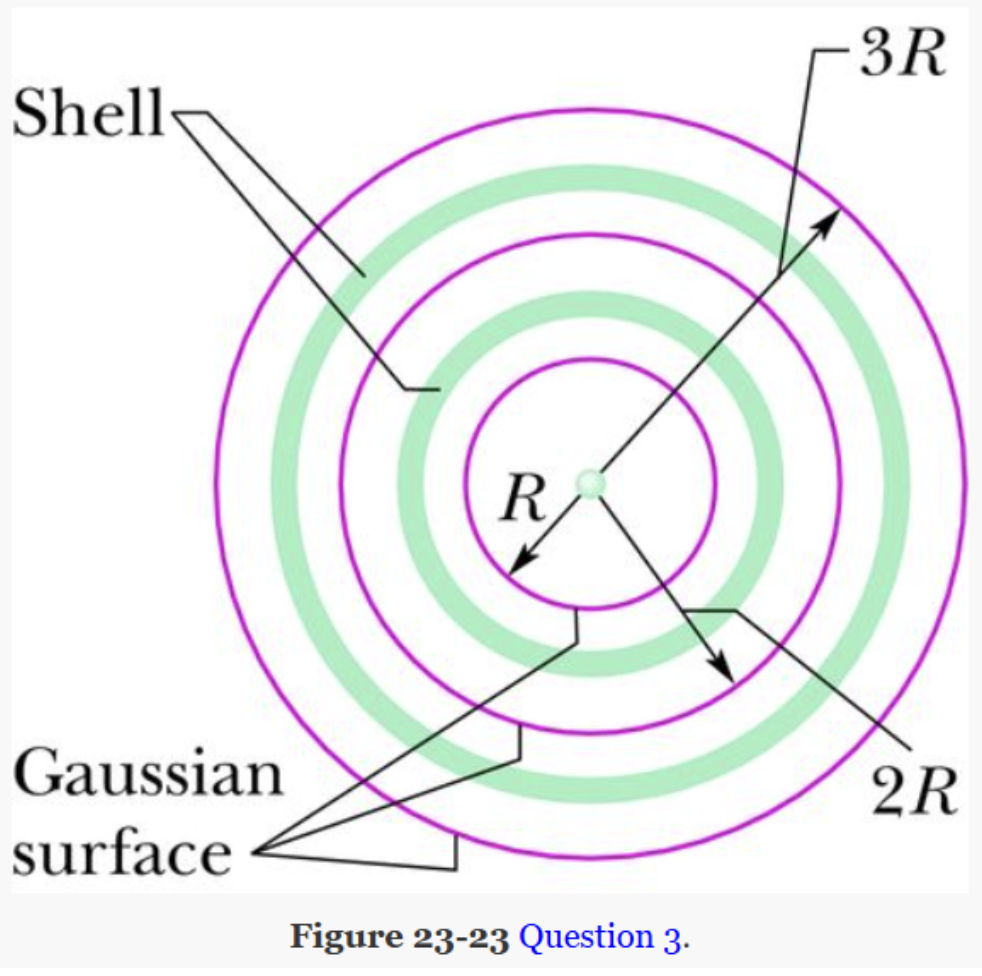
\includegraphics[width=0.5\textwidth]{picture_2.png} 
    % \label{fig:wrapfig}
\end{wrapfigure}
Figure 23-23 shows, in cross section, a central metal ball, two spherical metal shells, and three spherical Gaussian surfaces of radii R, 2R, and 3R, all with the same center. The uniform charges on the three objects are: ball, Q; smaller shell, 3Q; larger shell, 5Q. Rank the Gaussian surfaces according to the magnitude of the electric field at any point on the surface, greatest first.

\pagebreak
\section{Problem 6}
Three infinite nonconducting sheets, with uniform positive surface charge densities $\sigma$, $2\sigma$, and $3\sigma$, are arranged to be parallel like the two sheets in \text{\color{blue} Fig. 23-19a}. What is their order, from left to right, if the electric field $\vec{E}$ produced by the arrangement has magnitude $E = 0$ in one region and $E = 2\sigma/\epsilon_0$ in another region?

\subsection*{Solution}
For an infinite nonconducting sheet of densty $\sigma$, the electric field from it is equal to $E = \sigma/2\epsilon_0$. We can use this to provide a system of equations for electric field strengths $(a, b, c)$, which have unique magnitudes in the set $(\sigma/2\epsilon_0, 2\sigma/2\epsilon_0, 3\sigma/2\epsilon_0)$ or alternatively $(E, 2E, 3E)$. 
\begin{align*}
    a - b - c &= 0\\
    a + b - c &= 2\sigma/\epsilon_0 = 4E\\
    0a + 2b + 0c &= 4E\\
    b &= 2E = 2\sigma/2\epsilon_0\\
    a - 2E - c &= 0 \rightarrow a - c = 2E
\end{align*}

There is only one combination of the remaining two that this works for: $a = 3E$ and $c = E$. Thus, the order is \boxed{\langle 3\sigma, 2\sigma, \sigma \rangle}.

\pagebreak
\section{Problem 8}
\begin{wrapfigure}{r}{0.5\textwidth}
    \vspace{-30pt}
    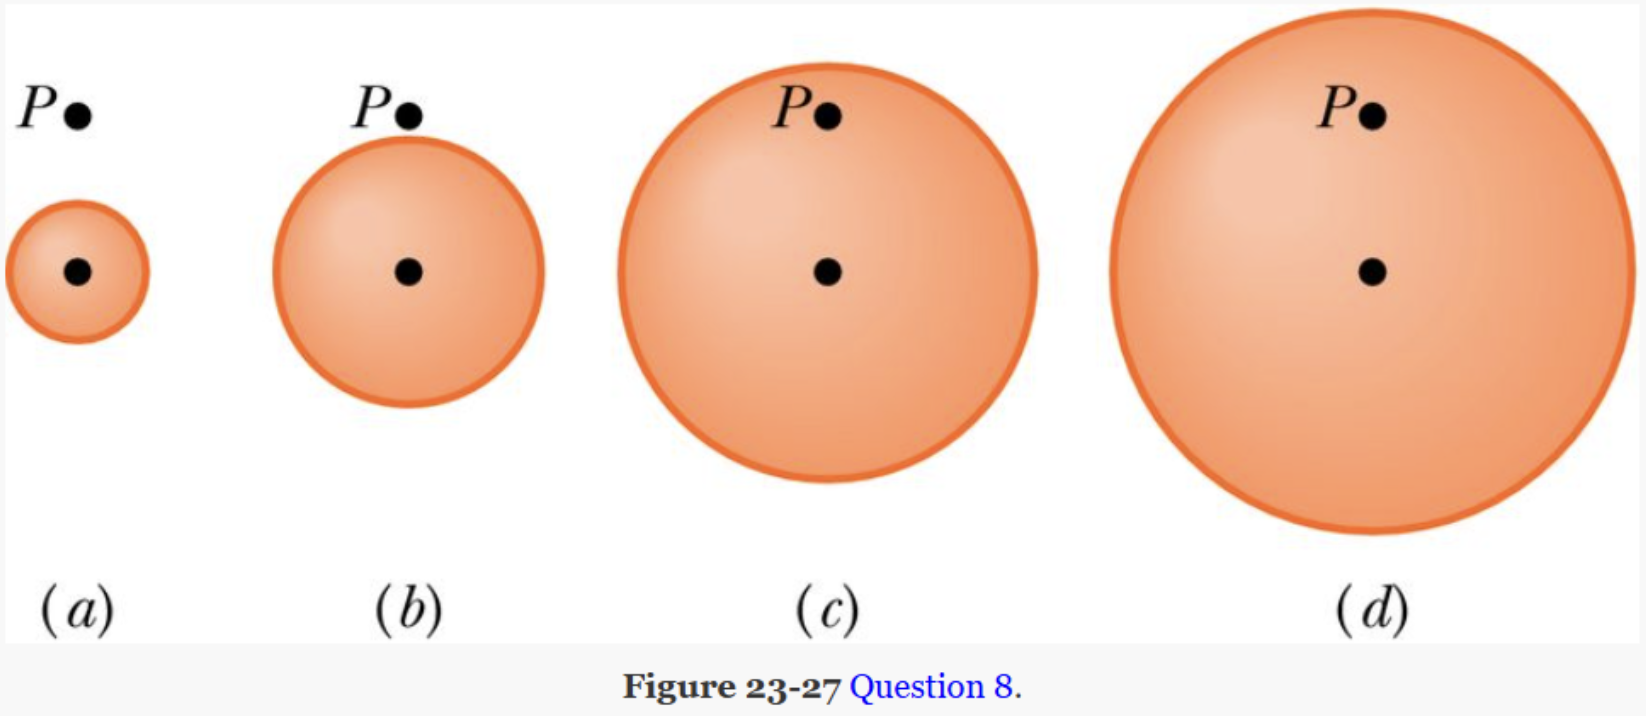
\includegraphics[width=0.5\textwidth]{picture_4.png} 
    % \label{fig:wrapfig}
\end{wrapfigure}

Figure 23-27 shows four solid spheres, each with charge $Q$ uniformly distributed through its volume. (a) Rank the spheres according to their volume charge density, greatest first. The figure also shows a point $P$ for each sphere, all at the same distance from the center of the sphere. (b) Rank the spheres according to the magnitude of the electric field they produce at point $P$, greatest first.

\subsection{Solution}
All have the same charge total and the spheres are charged uniformly. 
The charge density \(\rho\) of the sphere will be equal to the charge $Q$ divided by the volume $V$. 
The charge density can thus be ranked by the inverse of the volume and as such the inverse of the radius.
\boxed{(a) > (b) > (c) > (d)}

\subsection{Solution}
The electric field inside a solid sphere will be relevant for spheres (c) and (d). Know that anywhere on the sphere we are measuring the enclosure from, the electric field will be the same.
\begin{align*}
    \oint \vec{E} \cdot d\vec{A}    &=  \frac{Q_{enc}}{\varepsilon_0}\\
    E \int dA  &=  \frac{\rho \frac{4}{3}\pi P^3}{\varepsilon_0}\\
    E * 4\pi P^2    &=  \frac{4\pi P^3 \rho}{3 \varepsilon_0}\\
    E   &=  \frac{P \rho}{3 \varepsilon_0}
\end{align*}
The electric field outside a solid sphere (of radius $R$) will be relevant for spheres (a) and (b). Know that anywhere on the sphere we are measuring the enclosure from, the electric field will be the same.
\begin{align*}
    \oint \vec{E} \cdot d\vec{A}    &=  \frac{Q_{enc}}{\varepsilon_0}\\
    E \int dA   &=  \frac{\rho \frac{4}{3}\pi R^3}{\varepsilon_0}\\
    E * 4\pi P^2    &=  \frac{4\pi R^3 \rho}{3\varepsilon_0}\\
    E   &=  \frac{R^3 \rho}{3 P^2 \varepsilon_0}
\end{align*}
We have two equations, one for the electric field inside a uniformly charged sphere and other for the electric field outside the same. 
The value of P is the same for all four.
Since $\rho_c > \rho_d$, we can conclude that $E_c > E_d$.
Since $R_a < R_b$, we can conclude that $E_a < E_b$.
Additionally, since the electric field outside the sphere is a result of more charge than the electric field inside the sphere, $E_a > E_c$. 
As such, \boxed{E_b > E_a > E_c > E_d}.


\pagebreak
\section{Problem 10}
Figure 23-34 shows a closed Gaussian surface in the shape of a cube of edge length 2.00 m. It lies in a
region where the nonuniform electric field is given by E = (3.00x + 4.00)[ + 6.00f + 7.00K N/C with x in
meters. What is the net charge contained by the cube?

\section{Problem 12}
\begin{wrapfigure}{r}{0.5\textwidth}
    \vspace{-30pt}
    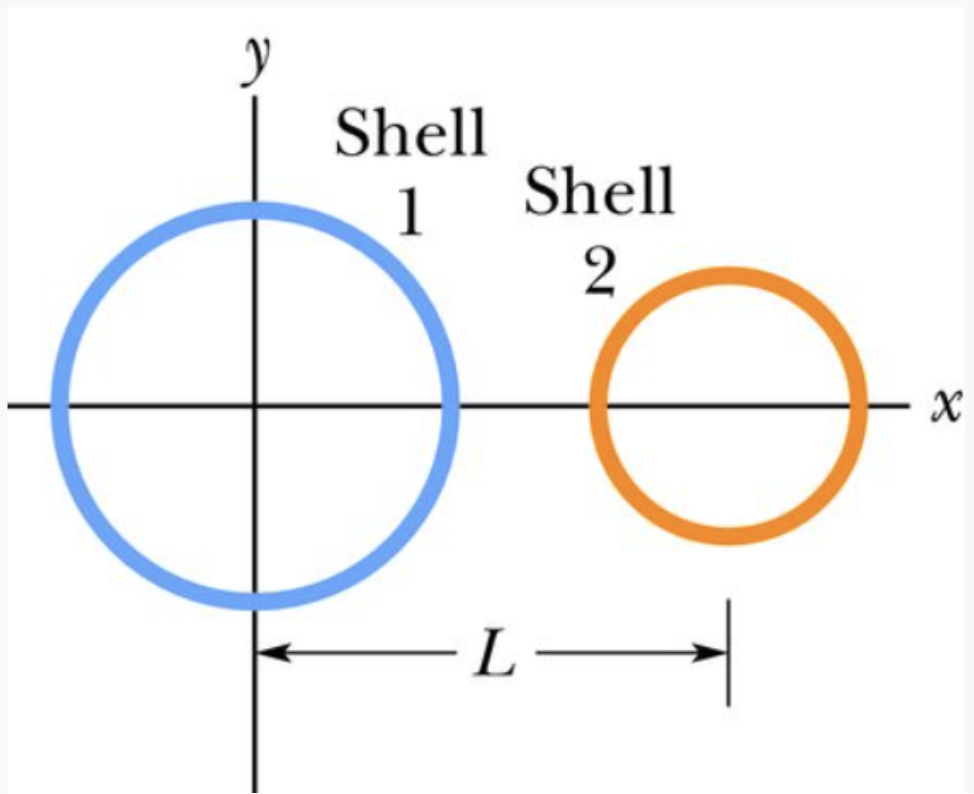
\includegraphics[width=0.5\textwidth]{picture_6.png} 
    % \label{fig:wrapfig}
\end{wrapfigure}
Figure 23-36 shows two nonconducting spherical shells fixed in place. Shell 1 has uniform surface
charge density $+6.0 \unit{\micro\coulomb/\meter}$ on its outer surface and radius $3.0 \unit{\centi\meter}$; shell 2 has uniform surface charge density $+4.0 \unit{\micro\coulomb/\meter}$ on its outer surface and radius $2.0 \unit{\centi\meter}$; the shell centers are separated by $L = 10 \unit{\centi\meter}$. In unit-vector notation, what is the net electric field at $x = 2.0 \unit{\centi\meter}$?

\section{Problem 18}
The electric field just above the surface of the charged conducting drum of a photocopying machine has a magnitude $E$ of $2.3 \times 10^5 \unit{\newton/\coulomb}$. What is the surface charge density on the drum?

\section{Problem 22}
An electron is released $9.0 \unit{\centi\meter}$ from a very long nonconducting rod with a uniform $6.0 \unit{\micro\coulomb/\meter}$. What is the magnitude of the electron's initial acceleration?

\subsection*{Solution}
We begin with the electric field of the electron at that point. We know the formula for the electric field along an infinite line of charge.
\begin{align*}
    E   &=  
\end{align*}

\section{Problem 28}
A charge of uniform linear density $2.0 \unit{\nano\coulomb/\meter}$ is distributed along a long, thin, nonconducting rod. The rod is coaxial with a long conducting cylindrical shell (inner radius = $5.0 \unit{\centi\meter}$, outer radius = $10 \unit{\centi\meter}$). The net charge on the shell is zero. (a) What is the magnitude of the electric field $15 \unit{\centi\meter}$ from the axis of the shell? What is the surface charge density on the (b) inner and (c) outer surface of the shell?

\subsection{Solution}
Electric field is not affected by things of zero charge, but it is affected by conducting things. Right outside the outer radius, the 

\pagebreak
\section{Problem 34}
\begin{wrapfigure}{r}{0.5\textwidth}
    \vspace{-30pt}
    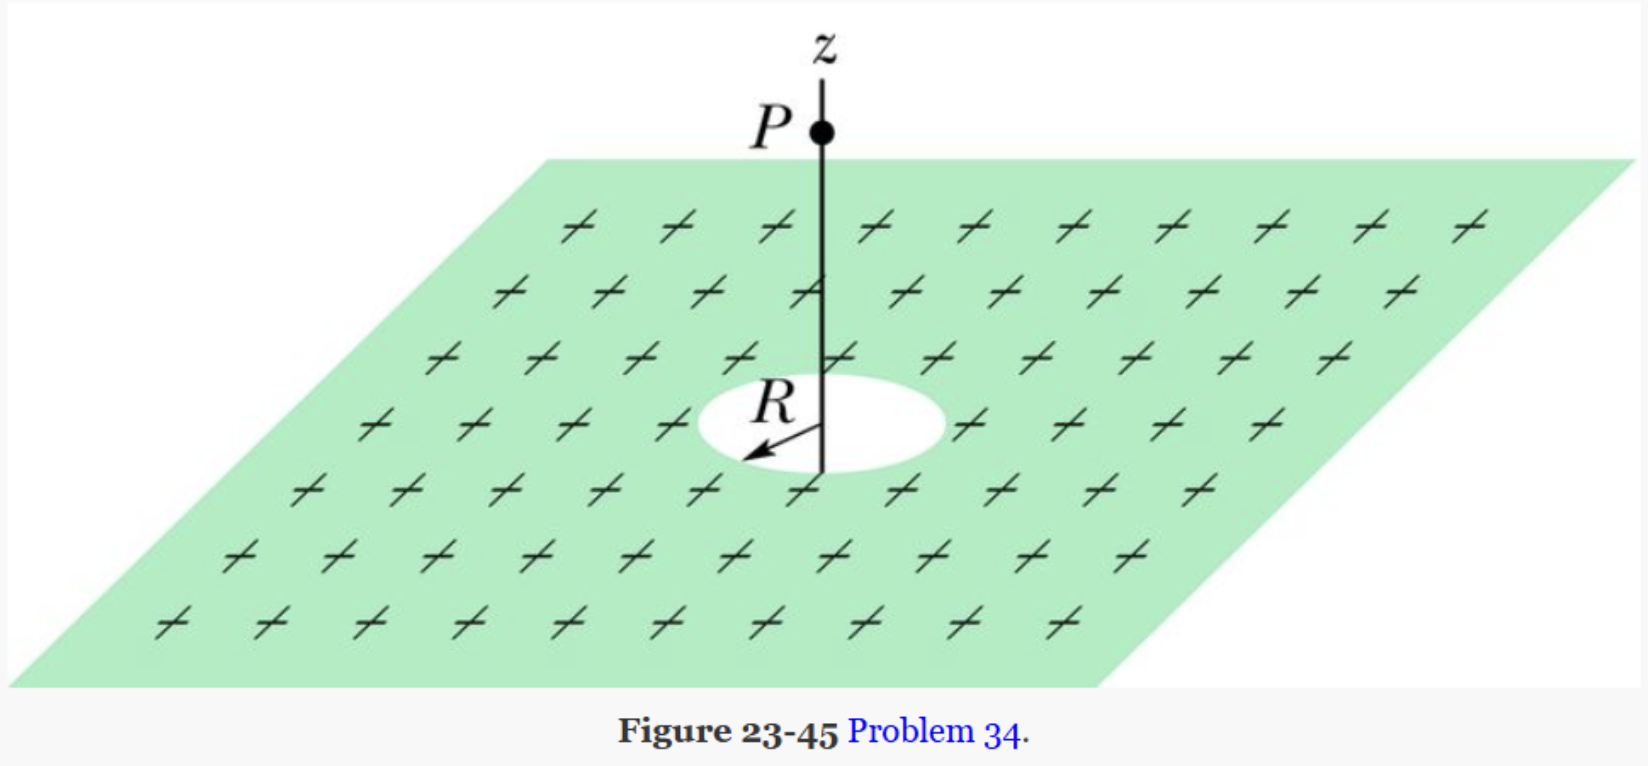
\includegraphics[width=0.5\textwidth]{picture_10.png} 
    % \label{fig:wrapfig}
\end{wrapfigure}
In \text{\color{blue} Fig. 23-45}, a small circular hole of radius $R = 1.80 \unit{\centi\meter}$ has been cut in the middle of an infinite, flat, nonconducting surface that has uniform charge density $\sigma = 4.50 \unit{\pico\coulomb/\meter^2}$. A $z$ axis, with its origin at the hole's center, is perpendicular to the surface. In unit-vector notation, what is the electric field at point $P$ at $z = 2.56 \unit{\centi\meter}$? (Hint: See Eq. 22-26 and use superposition.)

\subsection*{Solution}
As suggested, we use an equation and superposition. We know the formula for an infinite charged plane and a charged plate. We can add these together, keeping in mind that the plate's charge would be opposite the plane's.
\begin{align*}
    E_\Sigma    &=  E_{plane} - E_{plate}
        =   \frac{\sigma}{2\varepsilon_0} - \frac{\sigma}{2\epsilon_0} \left(1 - \frac{z}{\sqrt{z^2 + R^2}}\right)\\
        &=  \cancel{\frac{\sigma}{2\varepsilon_0}} - \cancel{\frac{\sigma}{2\epsilon_0}} + \frac{\sigma}{2\epsilon_0}\cdot\frac{z}{\sqrt{z^2 + R^2}}
        = \frac{\sigma}{2\epsilon_0}\cdot\frac{z}{\sqrt{z^2 + R^2}}
\end{align*}

We then can substitute in the known values.
\begin{align*}
    E_\Sigma    &=  \frac{\sigma}{2\epsilon_0}\cdot\frac{z}{\sqrt{z^2 + R^2}}\\
        &=  \frac{4.50 \times 10^{-12} \unit{\coulomb/\meter}}{2\varepsilon_0} \cdot \frac{2.56 \times 10^{-2} \unit{\meter}}{\sqrt{\left(2.56 \times 10^{-2} \unit{\meter}\right)^2 + \left(1.80 \times 10^{-2} \unit{\meter}\right)^2}}\\
        &=  \frac{4.50 \times 10^{-12}}{17.70 \times 10^{-12}} \cdot \frac{2.56 \times 10^{-2}}{\sqrt{9.7936 \times 10^{-4}}} \unit{\newton/\coulomb}\\
        &=  \frac{4.50*2.56}{17.70*3.1294} \unit{\newton/\coulomb}
        =   \frac{11.52}{55.39} \unit{\newton/\coulomb}
        =   0.208 \unit{\newton/\coulomb}
\end{align*}

Since it is in the $+z$ direction, we would have the final answer be \boxed{\boxed{0.208\hat{k}\ \unit{\newton/\coulomb}}}

\end{document}